\documentclass[10pt,pdflatex,headrule,landscape]{beamer}
\setbeamertemplate{caption}[numbered]

\setbeamertemplate{bibliography item}[text]

\usepackage{psfrag}
\usepackage{graphics,wrapfig,lipsum}
\usepackage{subfig}
\usepackage{graphicx}
\usepackage{color}
\usepackage{epsf}
\usepackage[english]{babel}
\usepackage{times}
\usepackage{amssymb}
\usepackage{amsmath}
\usepackage{amsfonts}
\mode<presentation> {
\usetheme{Warsaw}
\usecolortheme{seahorse}
\usecolortheme{rose}
\usefonttheme{professionalfonts}
}
\usepackage{mathtools}
\newcommand\vecnot[1]{\boldsymbol{#1}}
\newcommand\optvecnot[1]{\vecnot{#1}_{opt}}
\author{
Yehezkel Karo Itay\\[1cm]{Supervisor: Prof. Cohen Israel}\\{external supervisor: Dr. Dvorkind Tsvi}
}
\title{Feedback Based Spatial Beam-forming with Applications to Acoustic Signal Processing}

\institute[SFU]{
Department of Electrical Engineering \\
Technion - Israel Institute of Technology \\
Technion City, Haifa 3200003, Israel
}
\date[]

\newtheorem{property}{Property}[section]

\begin{document}

\begin{frame}
  \titlepage
\end{frame}

\begin{frame}
  \frametitle{Outline}
  \tableofcontents[hideallsubsections]
\end{frame}

\setlength{\parskip}{1em}

\section{Introduction}

\begin{frame}
\frametitle{Array processing}
Sensor array processing is a much studied subject.
\\
It has various implementations in multiple fields of research such as 
\begin{itemize}
 \item radar and sonar
 \item communication
 \item radio astronomy
 \item seismic science
 \item medical imaging and radiation
\end{itemize}
In particular, the uniform linear array (ULA), which consists of multiple equally spatially-spaced sensors (hence its name), is the basic, most studied array architecture.
\end{frame}

\begin{frame}
\frametitle{delay-and-sum beam-forming}
The most common basic beam-former is the delay-and-sum (Fig. \ref{fig:DelayAndSum}) which consists of weighted-and-summed ULA output signals which generates a spatially directed "beam" (Fig. \ref{fig:SimpleSpatialResponse}).
\begin{figure}%
    \centering
    \subfloat
    [Basic delay and sum architecture]
    {
    {
    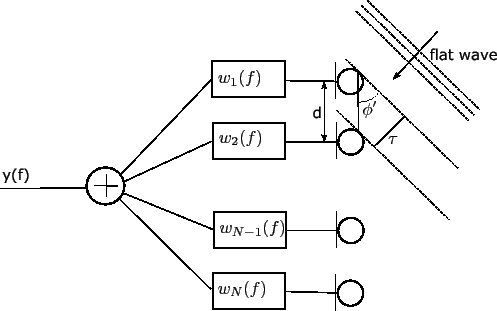
\includegraphics[width=0.35\textwidth]
    {Media/delay_and_sum_architecture.png}
    }
    \label{fig:DelayAndSum}
    }    
    \qquad
    \subfloat
    [Basic spatial response]
    {
    {
    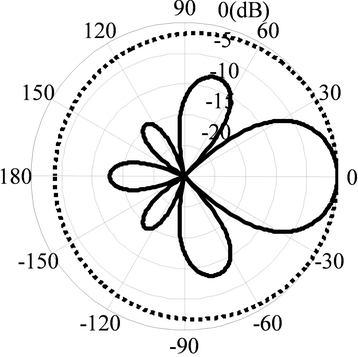
\includegraphics
    [width=0.2\textwidth]
    {Media/simple_spatial_response.PNG}
    }
    \label{fig:SimpleSpatialResponse}
    }
    \caption{Delay-and-sum filter and its spatial response.}
    \label{fig:delayAndSumArchAndResponse}    
\end{figure}
\end{frame}

\begin{frame}
\frametitle{signal processing fundamentals - filters}
\begin{itemize}
\item{
A filter is a linear system, consists of delay, gain and sum elements. The quantity of them in a specific filter is referred as ``resource usage''.
}
\item{
A filter can be described by its impulse response.
}
\end{itemize}
\end{frame}

\begin{frame}
\frametitle{Spatial filtering}
Filtering signals according to their spatial features (DOA) rather than their temporal features (frequency)
\begin{itemize}
\item 
{
\textbf{RX} : enabling better handling of interfering signals.
}
\item 
{
\textbf{TX} : enabling energy-efficient transmission.
}
\end{itemize}
\end{frame}

\begin{frame}
\frametitle{FIR vs. IIR}
\begin{minipage}{0.59\textwidth}
Filters can be divided to two main groups. 
\begin{itemize}
\item{
\textbf{Finite impulse response - FIR}
}
\item{
\textbf{Infinite impulse response - IIR}
}
\end{itemize}
\end{minipage}
\begin{minipage}{0.4\textwidth}
\begin{figure}
\centering
\subfloat
[Basic FIR filter architecture - simple delay, weight \& sum.]
{
{
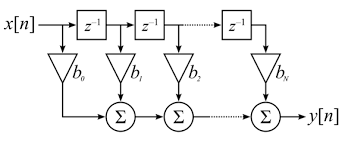
\includegraphics[width=0.9\textwidth]{Media/BASIC_FIR_FILTER_ARCH.png}
}
\label{fig:BasicFIRArch}
}
\qquad
\subfloat
[Basic IIR filter architecture - feedback based delay, weight \& sum.]
{
{
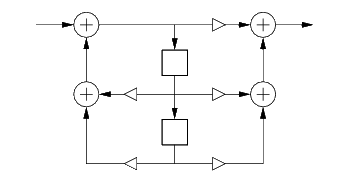
\includegraphics[width=0.8\textwidth]{Media/BASIC_IIR_FILTER_ARCH.png}
}
\label{fig:BasicIIRArch}
}
\caption{FIR vs. IIR architectures}
\label{fig:FIRvsIIRArch}
\end{figure}
\end{minipage}
\end{frame}

\begin{frame}
\frametitle{Why use IIR?}

\begin{itemize}
\item 
{
To achieve a wanted gain response, the IIR filter requires substantially fewer resources.
}
\item 
{
In array processing it means less antennas are needed.
}
\end{itemize}

\begin{figure}
\captionsetup{font={scriptsize},labelfont={scriptsize}}
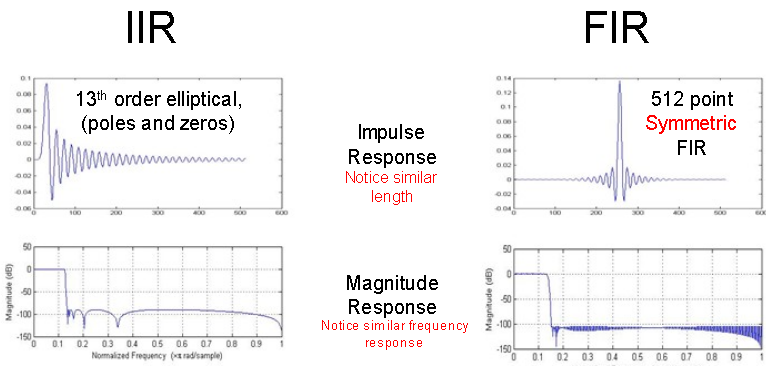
\includegraphics[width=.8\textwidth]{Media/FIRvsIIR.PNG}
% taken from : http://slideplayer.com/slide/6241667/
\caption{Resource usage difference between FIR and IIR of the gain response demands}
\end{figure}

\end{frame}

\begin{frame}
\frametitle{ULA as a spatial FIR}
\begin{minipage}{0.45\textwidth}
\begin{itemize}
\item{ULA of distance $ d $ between consecutive elements (signal DOA - $ \theta $)}
\item{FIR. Sampling interval $ \tau_{\theta}=\frac{d\cos{\theta}}{c} $ ($ c $ - propagation velocity)}
\end{itemize}
are similar \cite{van1988beamforming}.
\end{minipage}
\begin{minipage}{0.54\textwidth}
\begin{figure}
\captionsetup{font={scriptsize},labelfont={scriptsize}}
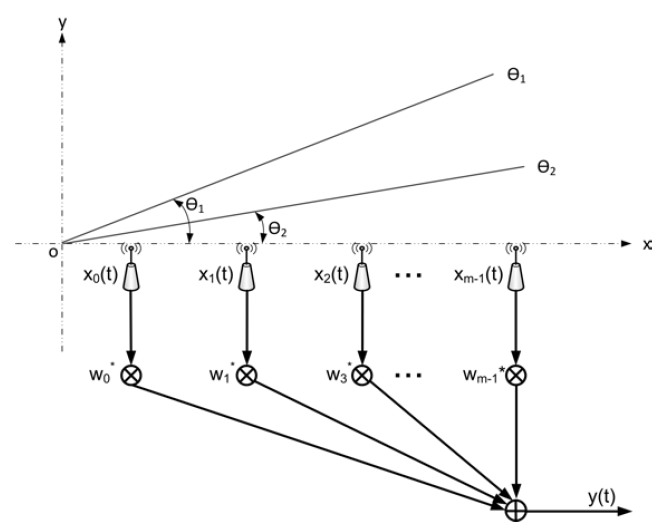
\includegraphics[width=\textwidth]{Media/ULA_FIR_similarity.PNG}
\caption{ULA and FIR similarity}
\end{figure}
\end{minipage}
\end{frame}

\section{Research goal}

\begin{frame}
\frametitle{Research main goal - Spatial \textbf{IIR}?}

\noindent
\makebox[0pt][l]{
\raisebox{-.9\totalheight}[0pt][0pt]{
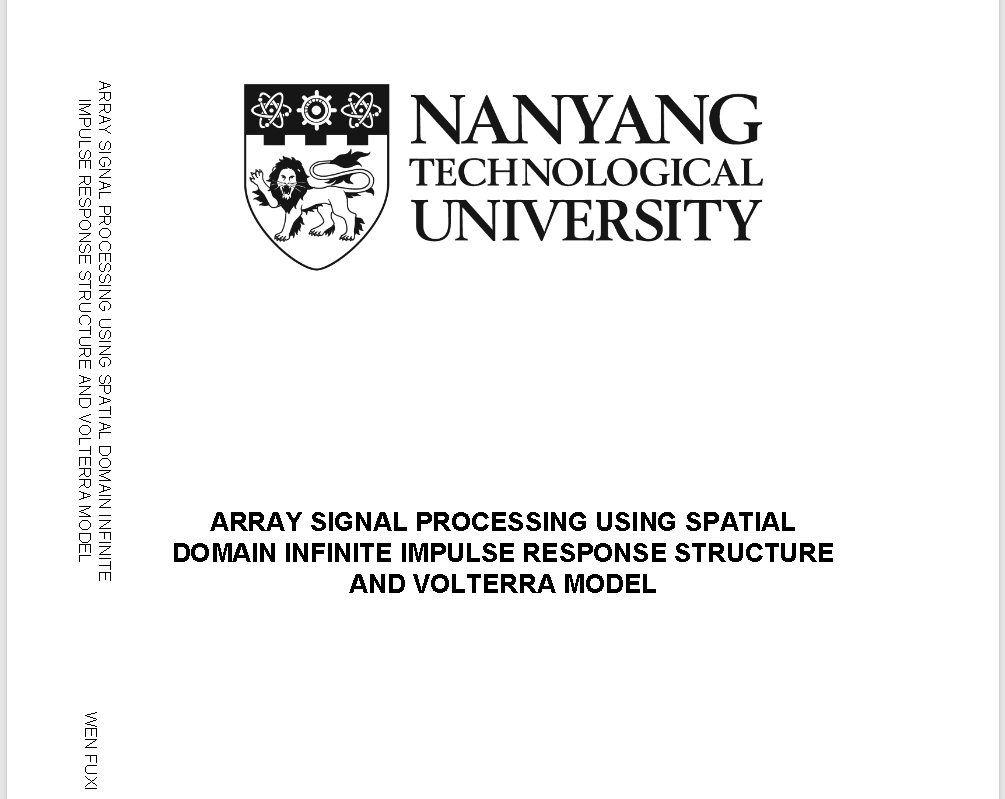
\includegraphics[width=.7\textwidth,angle=45]{Media/WensFrontPage.PNG}
}
}
\begin{itemize}
\item{
\colorbox{white}
{\parbox{\dimexpr\linewidth-2\fboxsep}{\strut \textbf{
``What is the array structure in spatial domain which is analogous to IIR filtering in the time domain?'' \cite{wen2013array}.
}\strut}}
}
\item{
\colorbox{white}
{\parbox{\dimexpr\linewidth-2\fboxsep}{\strut Our research can be referred as a further development of the PhD thesis of Wen.\strut}} 
}
\end{itemize}


\label{frm:ResearchMainGoal_SpatialIIR}
\end{frame}

\begin{frame}
\frametitle{Previously proposed methods for achieving ``Spatial-IIR'' - 1/4}
Some interesting methods were proposed in other papers \cite{wen2013array,Madanayake2008ABeamformer,Madanayake2009SystolicWDFs,Madanayake2008AFilters,Bruton2003Three-dimensionalBanks,Ward1986ABeamforming,Joshi2012SynthesisApplications} for achieving ``Spatial-IIR'' but none of them truly achieved the IIR response solely in the spatial (i.e. $ \theta $) domain.
\end{frame}

\begin{frame}
\frametitle{Previously proposed methods for achieving ``Spatial-IIR'' - 2/4}
\begin{minipage}{0.55\textwidth}
\begin{itemize}
\item
{
Estimate $ \theta $ and approximate $ \tau_{\theta} $ accordingly for the feedback part of the IIR. 
}
\end{itemize}
\end{minipage}
\begin{minipage}{0.44\textwidth}
\begin{figure}
\captionsetup{font={scriptsize},labelfont={scriptsize}}
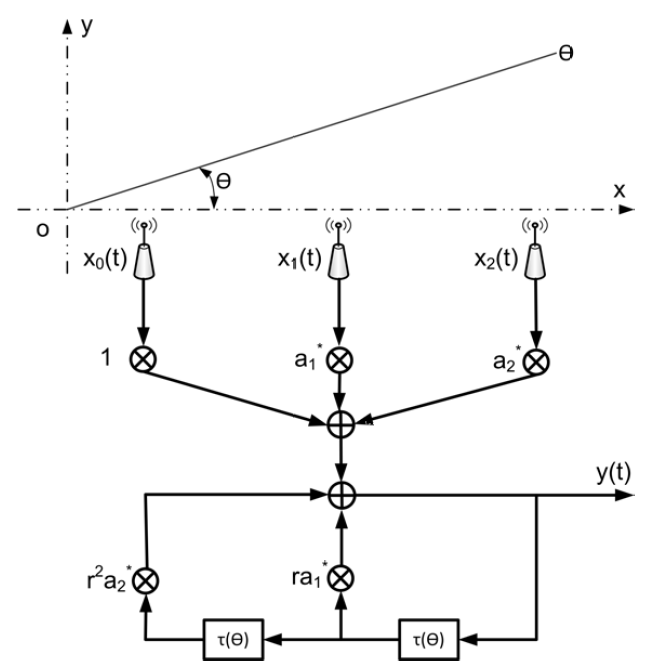
\includegraphics[width=\textwidth]{Media/WenFirstSuggestedMethod.PNG}
\caption{Wen's first suggested method - DOA estimation and approximated synthetic feedback delay.}
\end{figure}
\end{minipage}
\end{frame}


\begin{frame}
\frametitle{Previously proposed methods for achieving ``Spatial-IIR'' - 3/4}
\begin{minipage}{0.55\textwidth}
\begin{itemize}
\item
{
Using shifted sub arrays (see Fig.\ref{fig:ShiftedSubArraysWen}).
\\
Practically a complicated way for creating FIR response.
}
\end{itemize}
\end{minipage}
\begin{minipage}{0.44\textwidth}
\begin{figure}
\captionsetup{font={scriptsize},labelfont={scriptsize}}
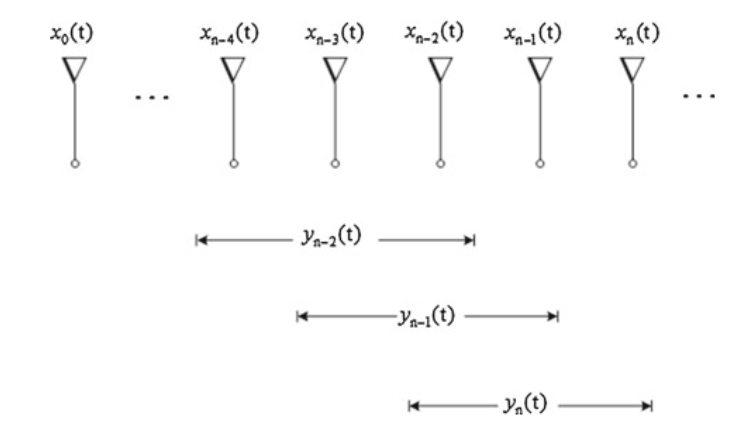
\includegraphics[width=\textwidth]{Media/SpatialIIR_SubArrays.PNG}
\caption{Shifted sub arrays to emulate IIR filter}
\label{fig:ShiftedSubArraysWen}
\end{figure}
\end{minipage}
\end{frame}

\begin{frame}
\frametitle{Previously proposed methods for achieving ``Spatial-IIR'' - 4/4}
\begin{minipage}{0.55\textwidth}
\begin{itemize}
\item
{
\textbf{2-D spatio-temporal filtering}
\begin{itemize}
\item{The wavefront is viewed as a two dimensional signal - space and time}
\item{Spatial FIR combined with temporal IIR}
\item{As can be seen in Fig.\ref{fig:SpatioTemporalPlaneWavePracticalFilter} taken from \cite{Bruton2003Three-dimensionalBanks}, the obtained 2-D filter is not ideal}
\end{itemize}
}
\end{itemize}
\end{minipage}
\begin{minipage}{0.44\textwidth}
\begin{figure}
\captionsetup{font={scriptsize},labelfont={scriptsize}}
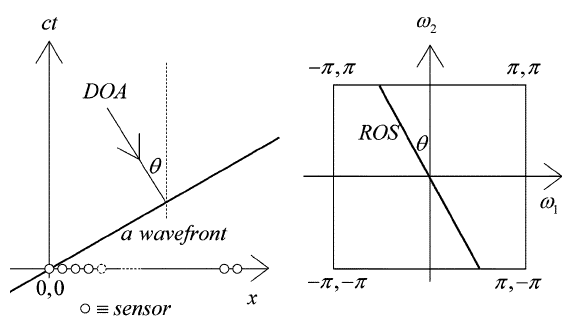
\includegraphics[width=\textwidth]{Media/SpatioTemporalPlaneWave.PNG}
\caption{\tiny{Spatio-temporal representation of plane wave}}
\label{fig:SpatioTemporalPlaneWave}
\end{figure}
\begin{figure}
\captionsetup{font={scriptsize},labelfont={scriptsize}}
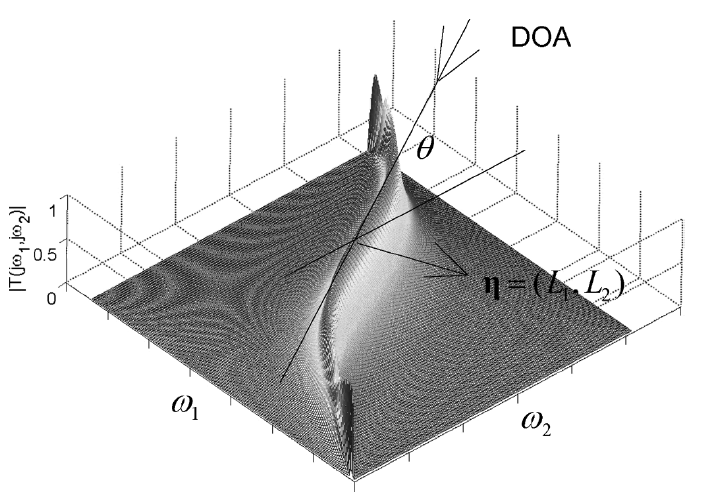
\includegraphics[width=.6\textwidth]{Media/SpatioTemporalPlaneWavePracticalFilter.PNG}
\caption{\tiny{Practical spatio-temporal 2D plane-wave filter.}}
\label{fig:SpatioTemporalPlaneWavePracticalFilter}
\end{figure}
\end{minipage}
\end{frame}

\section{Signal model and problem formulation}

\begin{frame}
\frametitle{Signal Model - suggested system architecture}
\begin{minipage}{0.45\textwidth}
\textbf{Our suggested method}
\begin{itemize}
\item
{
Feedback based.
}
\item
{
Cooperative speaker - transmits a feedback signal, synthesized by our system, in addition to its own.
}
\item
{
As will be shown, achieves a spatial-only auto-regressive transfer function.
}
\end{itemize}
\end{minipage}
\begin{minipage}{0.44\textwidth}
\begin{figure}
\captionsetup{font={scriptsize},labelfont={scriptsize}}
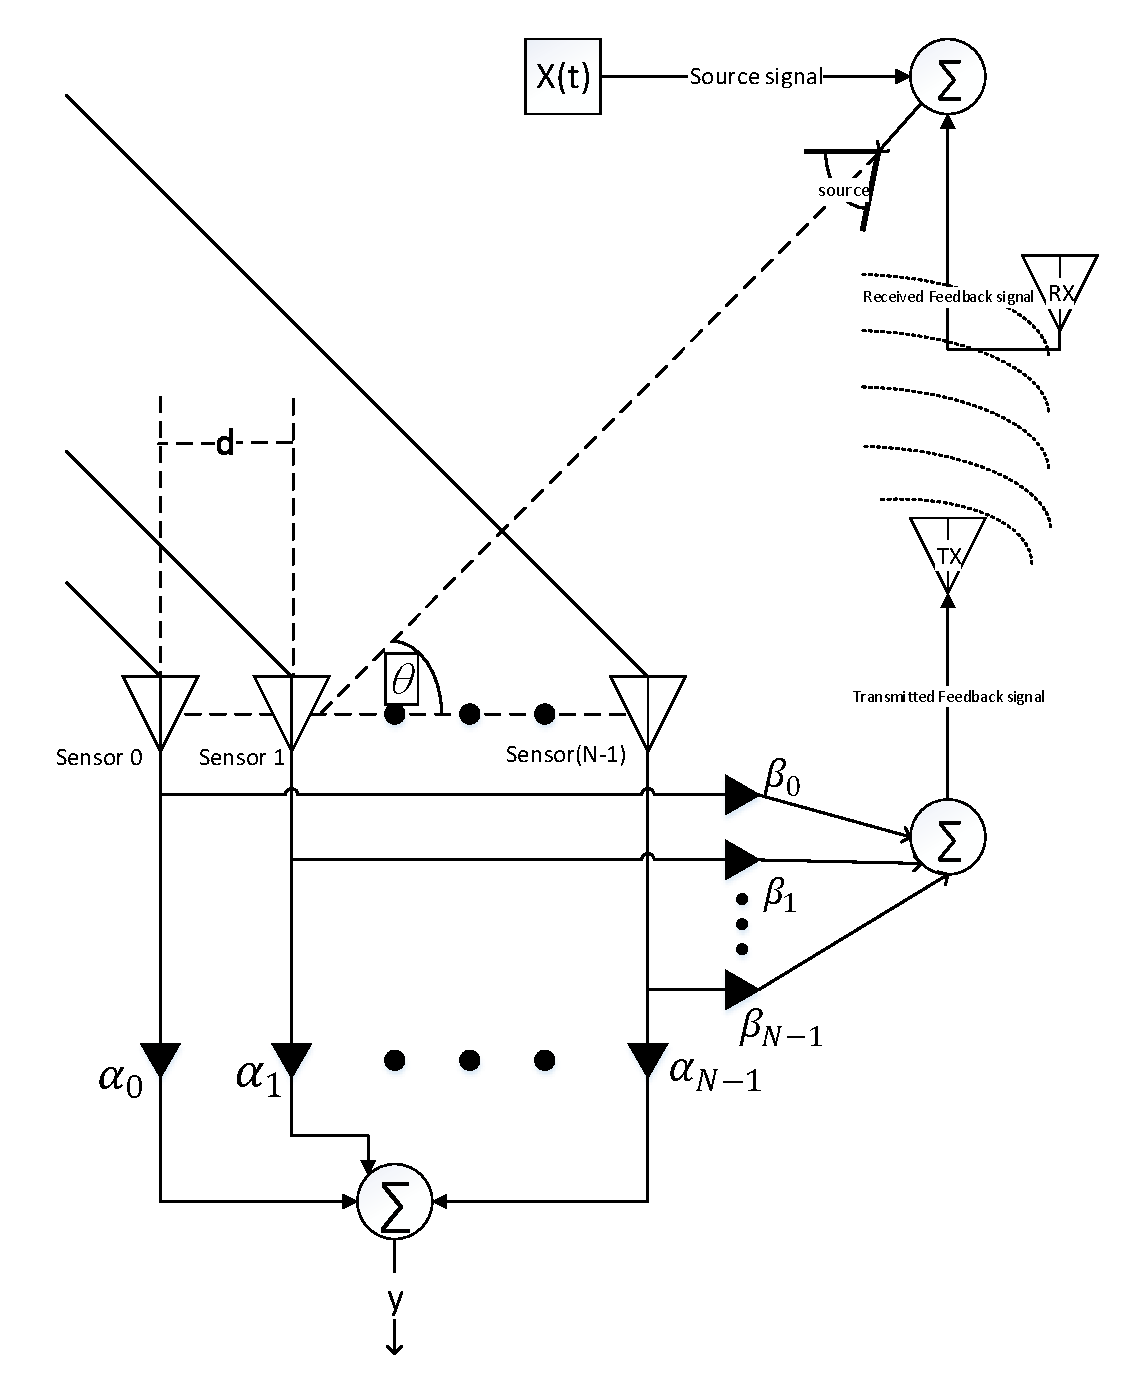
\includegraphics[width=\textwidth]{./Media/SpatialIIR-diagram/SpatialIIR_VER4.pdf}
\caption{Proposed system feedback-based architecture}
\label{fig:SpatialIIRSuggestedArch}
\end{figure}
\end{minipage}
\end{frame}

\begin{frame}[allowframebreaks]
\frametitle{Resolving the system transfer function}
Denoting:\\
$ x $ - source signal,\\
$ y $ - beamformer output,\\
$ \vecnot{\alpha},\vecnot{\beta} $ - user-controlled coefficient vectors,\\
$\vecnot{d}_{\theta}$ - steering vector with n'th element $e^{-j\omega \tau_{n,\theta}}$,\\
$ \tau_{pd} $ - propagation delay from the source to the reference sensor,\\
$ \tau_{tx} $ - feedback transmission delay\\
and assuming a simple flat channel, the equation which defines the \textbf{received signal at the n'th sensor}, and due to a wavefront from DOA $\theta$ is 
$$
x_{n,\theta}(t) = x(t-\tau_{pd}-\tau_{n,\theta})+\sum_{m=0}^{N-1}{\beta_{m}x_{m,\theta}(t-\tau_{pd}-\tau_{tx}-\tau_{n,\theta})}
$$
which, after taking all the array elements into account converts to
$$
\ifdefined\DEFIncludeAttenuation
    y^{\mathcal{F}}_{\theta}(\omega) 
    = 
    \vecnot{\alpha}^{T}
    \left(
    I
    -g^{2}\vecnot{d}_{\theta}
    \vecnot{\beta}^{T}
    e^{-j\omega(\tau_{pd}+\tau_{tx})}
    \right)
    ^{-1}
    g^{2}
    \vecnot{d}_{\theta}
    x^{\mathcal{F}}(\omega)
    e^{-j\omega\tau_{pd}}
\else
    y^{\mathcal{F}}_{\theta}(\omega) 
    = 
    \vecnot{\alpha}^{T}
    \left(
    I
    -\vecnot{d}_{\theta}
    \vecnot{\beta}^{T}
    e^{-j\omega(\tau_{pd}+\tau_{tx})}
    \right)
    ^{-1}
    \vecnot{d}_{\theta}
    x^{\mathcal{F}}(\omega)
    e^{-j\omega\tau_{pd}}
\fi
$$
under the Fourier transform.
\\
Using the Woodbury matrix identity \cite{woodbury1950inverting} yields
$$
\ensuremath{
y_{\theta}^{\mathcal{F}}(\omega) 
=
\frac
{
\vecnot{\alpha}^{T}
\vecnot{d}_{\theta}
exp\left(-j\tau\right)
}
{
1
-
\vecnot{\beta}^{T}\vecnot{d}_{\theta}
exp\left(-j\tau\right)
}
x^{\mathcal{F}}(\omega)
}
$$
and if we define $e^{-j\omega \tau_{n,\theta}} \equiv z $, $\vecnot{d}_{\theta}$ can be viewed as the integer powers of z vector and the transfer function becomes a regular digital filter's functions with configurable $ \vecnot{\alpha},\vecnot{\beta} $ coefficients.

\end{frame}

\section{Research tasks \& hurdles}

\begin{frame}
\frametitle{Previous intended tasks}
Previous defined objectives were:
\begin{itemize}
\item
{
Develop a method for choosing the optimal coefficients for $ \vecnot{\alpha},\vecnot{\beta} $.
}
\item
{
Study the system's stability properties.
}
\item
{
Implement a real world demo.
}
\end{itemize}
\end{frame}

\begin{frame}
\frametitle{Research tasks - progress update (I)}
\begin{minipage}{0.45\textwidth}
\begin{itemize}
\item
{
Study the system's stability properties.
\begin{itemize}
\item{
Feedback delay causes the system poles to ``travel'' in the $ Z $ plane.
}
\item{
Even a slight (millimeters) error in the range ($ \tau_{pd} $) estimation can cause a very significant phase error in the system's denominator.
}  
\end{itemize}
}
\end{itemize}
\end{minipage}
\begin{minipage}{0.5\textwidth}
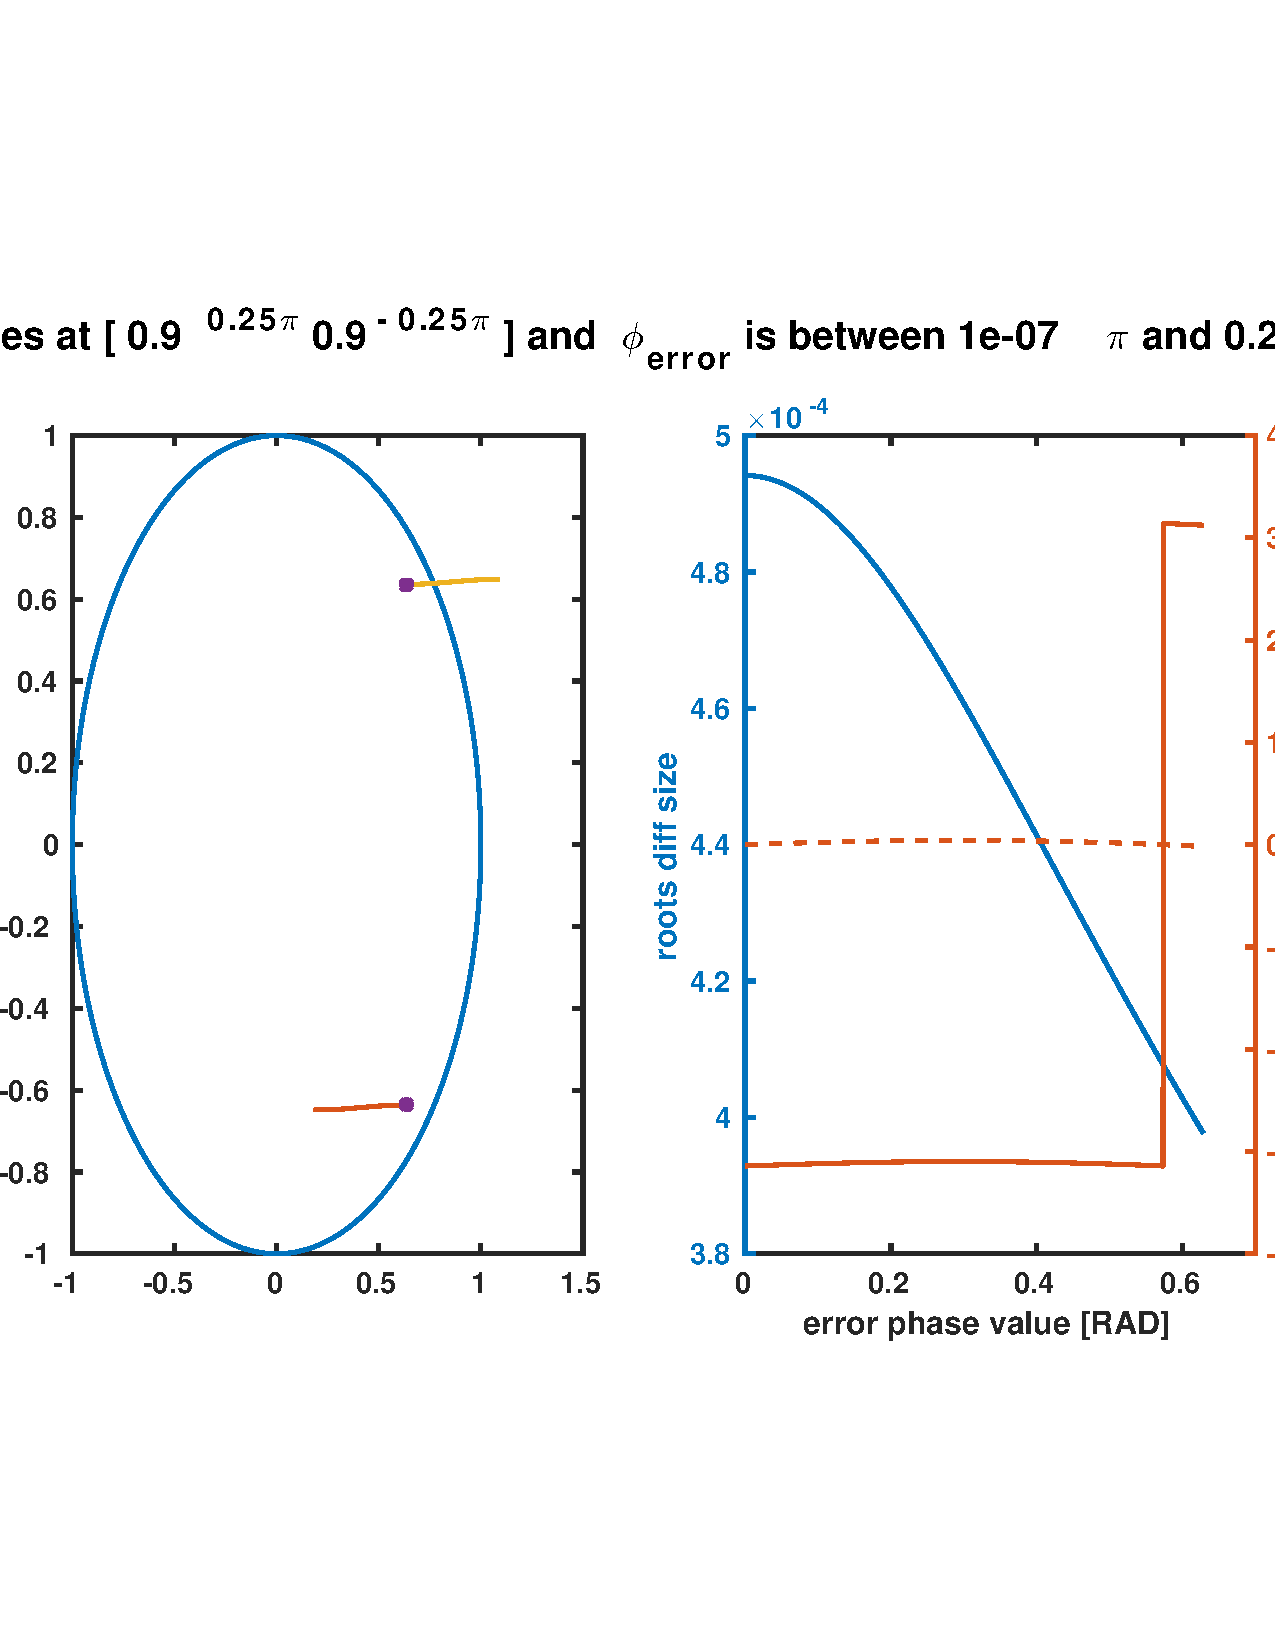
\includegraphics[width=\textwidth]{Media/notchRootLocus.pdf}
\end{minipage}
\end{frame}

\begin{frame}
\frametitle{Research tasks - progress update (II)}
The other tasks are dependent in the solving of the stability issue:
\begin{itemize}
\item
{
Develop a method for choosing the optimal coefficients for $ \vecnot{\alpha},\vecnot{\beta} $.
}
\item
{
Implement a real world demo.
}
\end{itemize}
\end{frame}

\begin{frame}
\frametitle{Stability issue solving trials (I)}
Until now we considered various approaches for solving the stability issue:
\begin{itemize}
\item
{
\textbf{Robust filter design}
\\
Robust digital IIR design methods \cite{Agarwal1975NewNoise,Li1993RoundoffRealizations,Kauraniemi1998DeltaFilters} dictate the use of integrators, which leads back to the main problem.
}
\item
{
\textbf{Solving an optimization problem}
\\
\begin{equation*}
\begin{aligned}
& \underset{\vecnot{\alpha},\vecnot{\beta}}{\text{minimize}}
& & 
\left\lVert 
H_{d}(\theta) - H_{\vecnot{\alpha},\vecnot{\beta},\phi}(\theta)
\right\rVert^p
\\
& \text{subject to}
& & 0 < \phi \leq 2\pi, \; i = 1, \ldots, m.
\end{aligned}
\end{equation*}
where 
$ 
H_{\vecnot{\alpha},\vecnot{\beta},\phi}(\theta) =  
\frac
{
\vecnot{\alpha}^{T}
\vecnot{d}_{\theta}
}
{
1
-
\vecnot{\beta}^{T}\vecnot{d}_{\theta}
e^{-j\phi}
}
$
and 
$ 
H_{d}(\theta) =  
\frac
{
\vecnot{\alpha_{d}}^{T}
\vecnot{d}_{\theta}
}
{
\vecnot{\beta}_{d}^{T}\vecnot{d}_{\theta}
}
$
}
\end{itemize}
\end{frame}

\begin{frame}
\frametitle{Stability issue solving trials (II)}
\begin{itemize}
\item{
\textbf{Synthetic sync signal broadcast}
\\
Insert a synthetic signal of constant frequency to the system and iteratively modifying the phases of the feedback coefficient.
}
\item{
\textbf{Adapting control theory methods}
\\
``Networked Controlled System'' \cite{Luan2011StabilizationDelays,Lewis1998ControlDelays} 
\\
Control-via-network where the sensor delay is random.
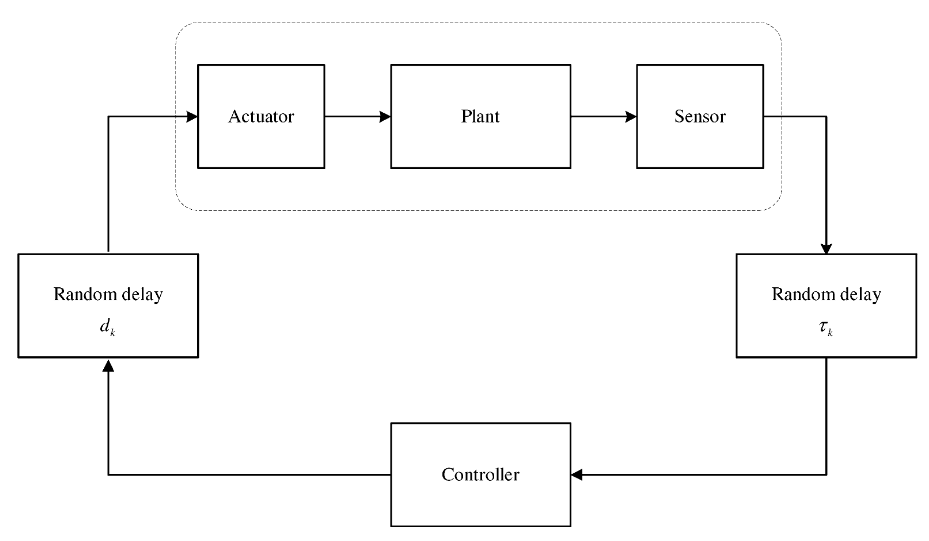
\includegraphics[width=.6\textwidth]{Media/networkedControl.PNG}
}
\end{itemize}
\end{frame}

\section{Conclusion}

\begin{frame}
\frametitle{Future plans}
Our next objectives are
\begin{itemize}
\item{Analytical examination of the notch filter sensitivity.}
\item{Range estimation CRLB calculation in a single speaker scenario.}
\item{Examine a two close-frequency feedback modulation method.}
\end{itemize}
\end{frame}


\begin{frame}[allowframebreaks]
\frametitle{References}
\bibliographystyle{unsrt}
\tiny{\bibliography{./Modules/Mendeley,./Modules/LocalBib}}
\end{frame}

\end{document}
